
\begin{frame}{tasks}
	\begin{itemize}
		\item Hardware auswaehlen
		\item SDK bauen
		\item Developer-Image erstellen
		\item services erstellen
		\item service auf Host testen
		\item Yocto rezept fuer service erstellen
		\item service in SDK installieren
		\item repeat
		\item image erstellen
		\item image deployen
	\end{itemize}
\end{frame}


\begin{frame}{system}
	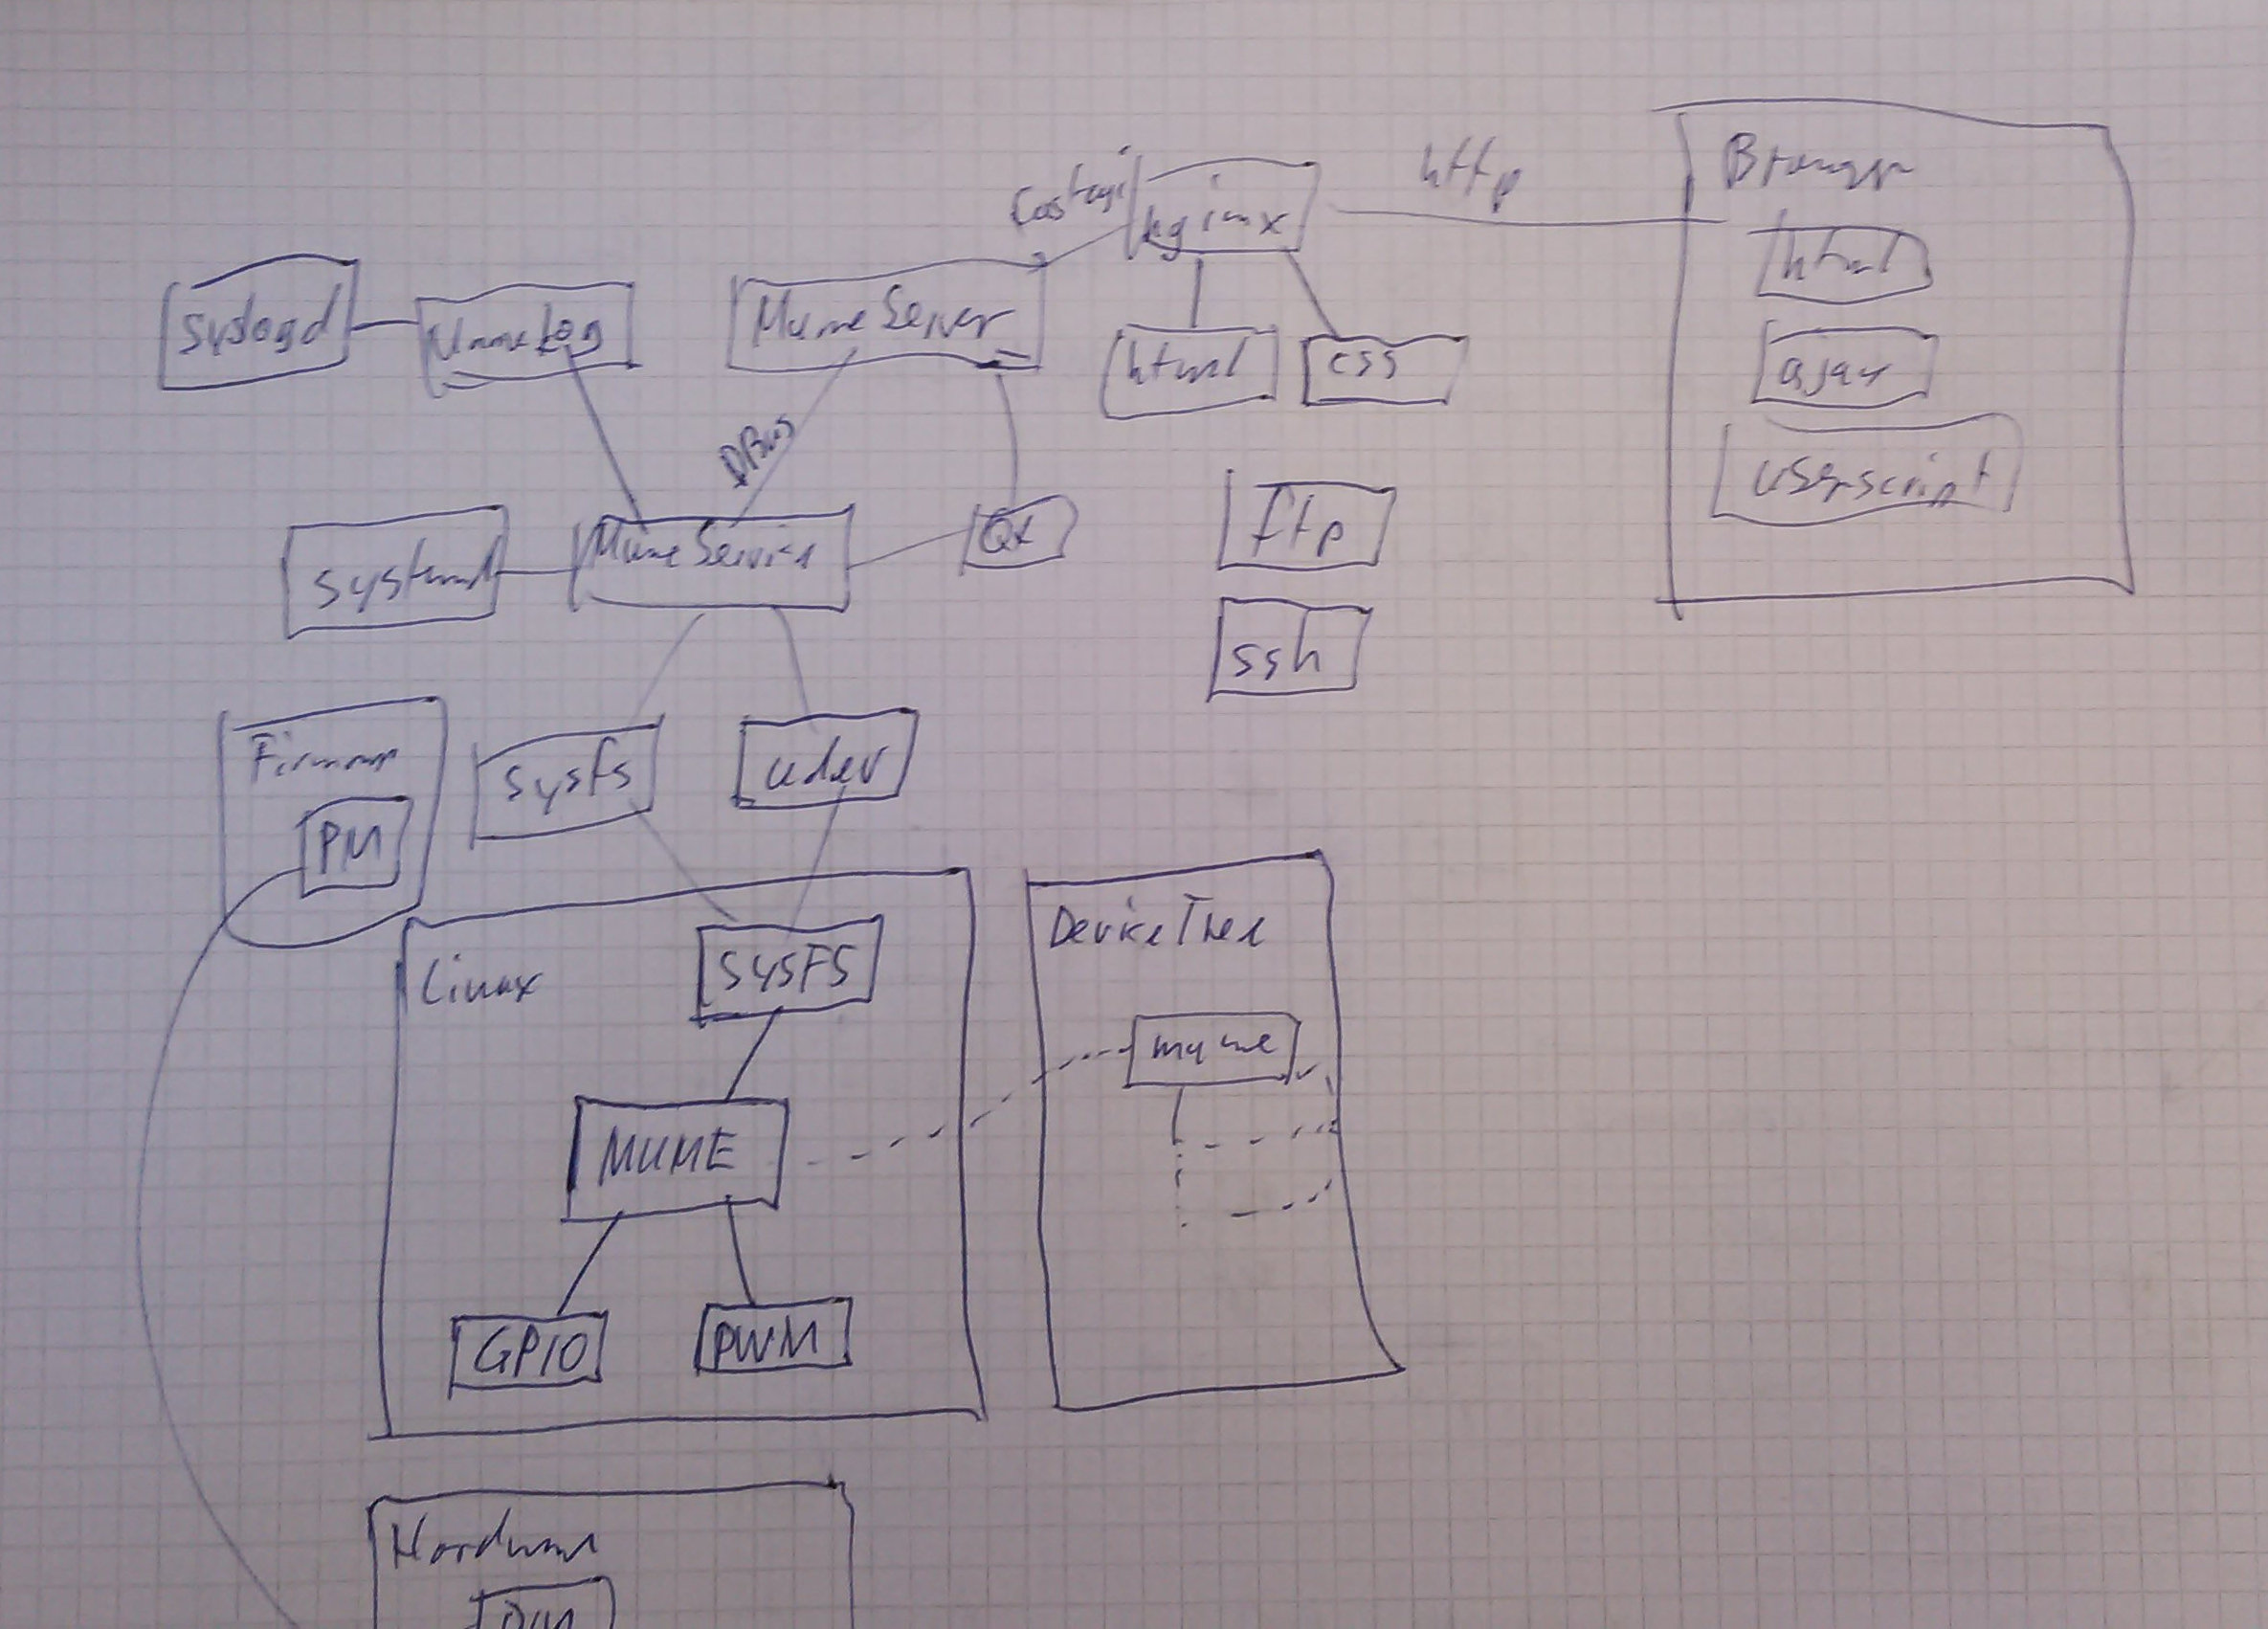
\includegraphics[width=\textwidth]{res/system.jpg}
\end{frame}

\begin{frame}{Linux}
	\begin{itemize}
		\item Sammlung von Subsystemen, abstraktionenen
		\item i2c
		\item spi
		\item iio
		\item fbtft
		\item gpio
		\item led
	\end{itemize}
\end{frame}

\begin{frame}{eigener Treiber}
	Beispiel ``Most Usless Machine Ever''
\end{frame}

\begin{frame}{Applikationen}
	Siehe System
	\begin{itemize}
		\item Embedded System besteht meist aus mehreren Prozessen $\rightarrow$ Microservices
		\item Webserver, Prozessueberwachung, SSH, FTP, UI
		\item gutes IPC system (z.B. kdbus)
		\item eigener Service
		\begin{itemize}
			\item reaktiv, event-getriggert
			\item Qt gut geeignet
			\item andere Frameworks moeglich
			\item auch ohne Framework moeglich
		\end{itemize}
	\end{itemize}
\end{frame}

\begin{frame}{Webserver}
\end{frame}